\documentclass{beamer}
\usepackage{tcolorbox}
\usepackage{mathtools}
\usepackage{notation} % Custom package
\usepackage{pgfplots}
\usepackage{amsmath}
\usepackage{amssymb}
\usepackage{pdfpages}

%\beamerdefaultoverlayspecification{<+->}
% \newcommand{\data}{\mathcal{D}}
% \newcommand\Item[1][]{%
% 	\ifx\relax#1\relax  \item \else \item[#1] \fi
% 	\abovedisplayskip=0pt\abovedisplayshortskip=0pt~\vspace*{-\baselineskip}}


\usetheme{metropolis}           % Use metropolis theme
\graphicspath{ {./SVM/} }

\title{SVM Soft Margin Classification}
\date{\today}
\author{Nipun Batra}
\institute{IIT Gandhinagar}
\begin{document}
	\maketitle
	
{
	\setbeamercolor{background canvas}{bg=}
	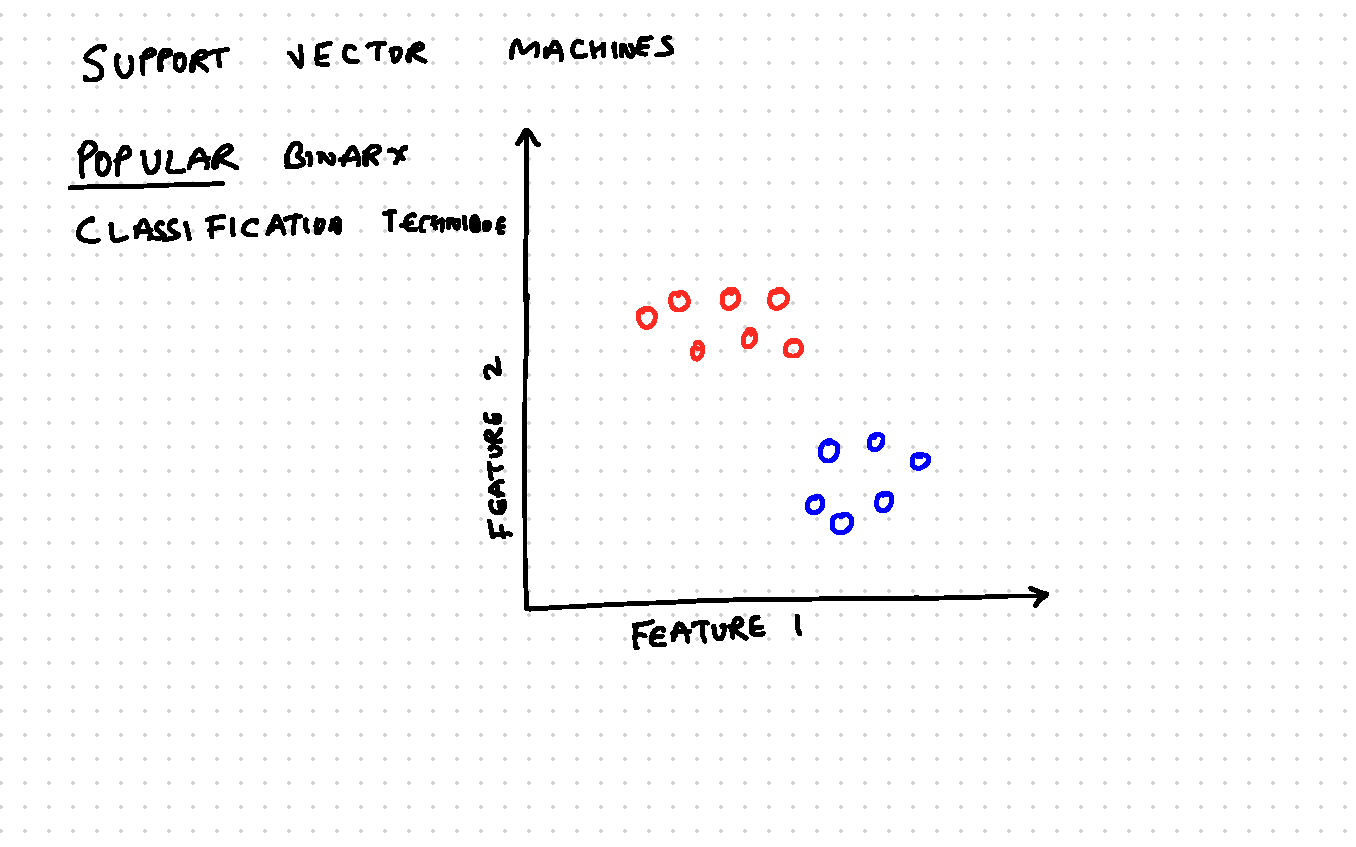
\includepdf[page=50]{Svm-notes.pdf}
}

	
	\begin{frame}{Soft-Margin SVM}
	\begin{itemize}[<+->]
		\item Can we learn SVM for ``slightly'' non-separable data without projecting to a higher space? 
		\item Introduce some ``slack'' ($\xi_i$) or loss or penalty for samples - allow some samples to be misclassified
		
	\end{itemize}
		
		
		
	\end{frame}

{
	\setbeamercolor{background canvas}{bg=}
	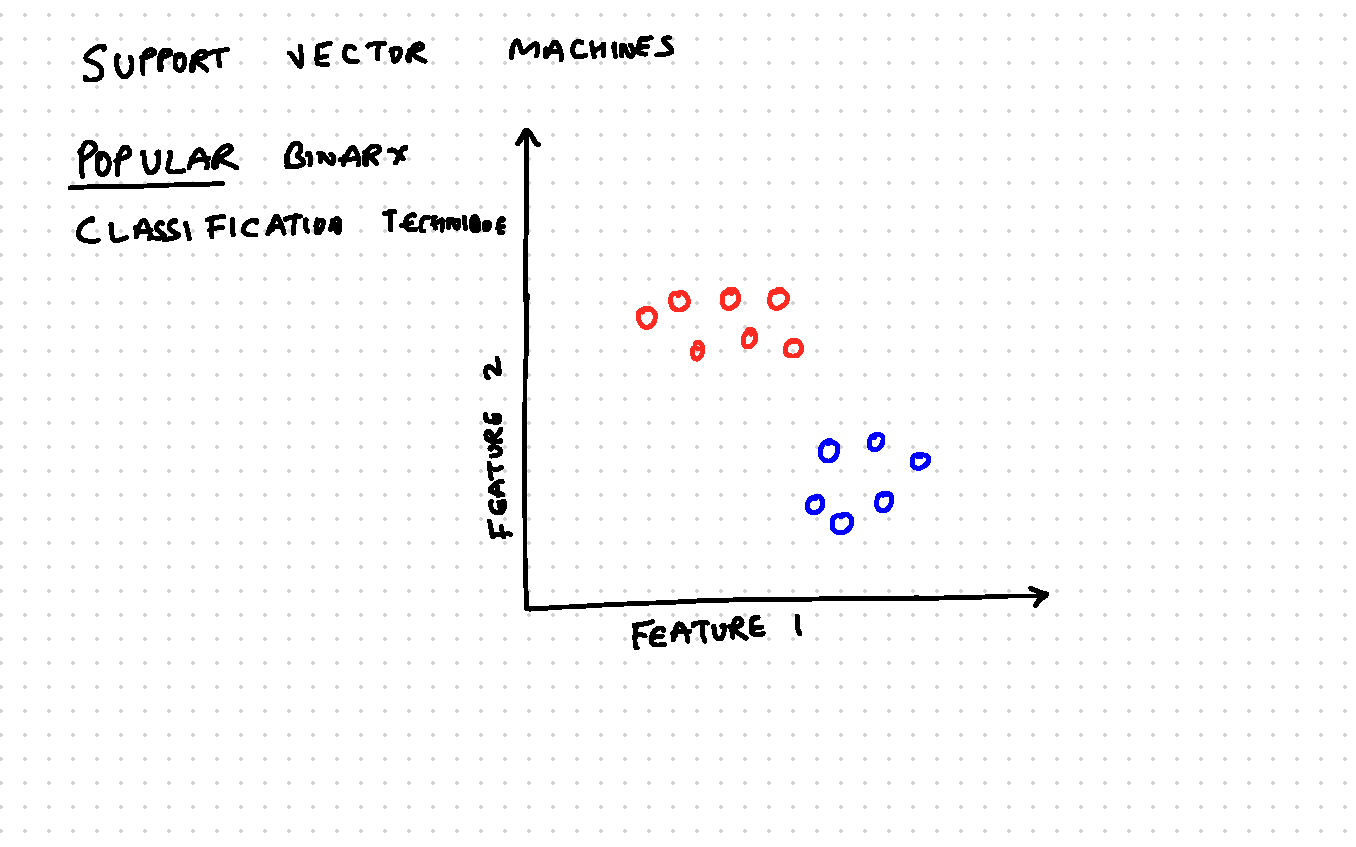
\includepdf[page=51-58]{Svm-notes.pdf}
}
	
	\begin{frame}{Soft-Margin SVM}
		Change Objective \\
		\vspace{0.1cm}
		$\min \frac{1}{2}\lvert\lvert\bar{w}\rvert\rvert^{2} + C \sum_{i=1}^{n}\xi_{i}$ \\ s.t. $y_{i}(\bar{w}\bar{x_i} + b) \geq 1 - \xi_{i}$ \\
		
		\vspace{0.2cm}
		\pause In Dual:
		$$\text{Minimize} \sum_{i=1}^{n}\alpha_{i} - \sum_{i=1}^{n}\sum_{j=1}^{n}\alpha_{i}\alpha_{j}y_{i}y_{j}\bar{x}_{i}\bar{x}_{j}$$
		s.t.
		$$0 \leq \alpha_{i} \leq C \text{\hspace{0.3cm}\&\hspace{0.3cm}} \sum_{i=1}^{n}\alpha_{i}y_{i} = 0$$
		
	\end{frame}


{
	\setbeamercolor{background canvas}{bg=}
	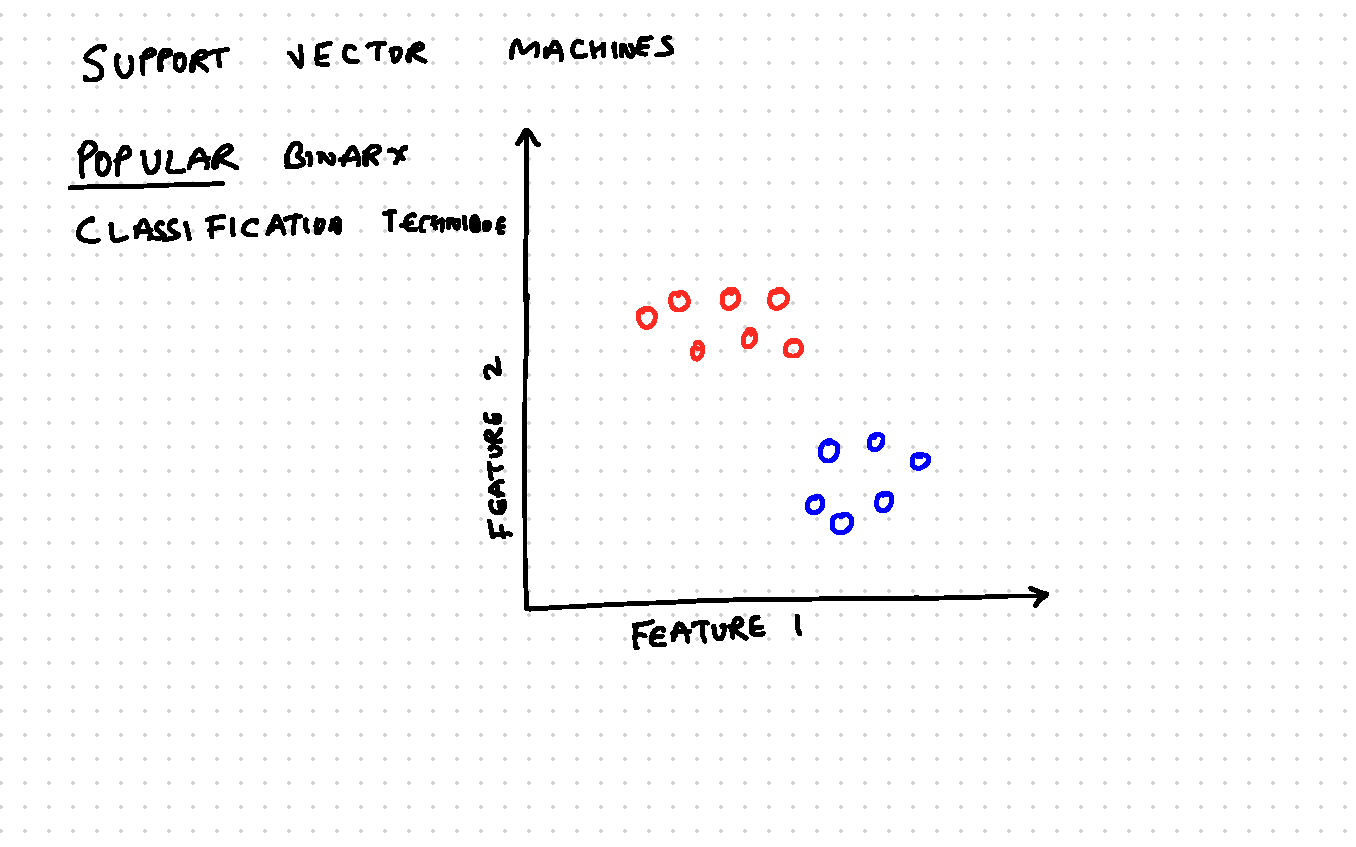
\includepdf[page=59-61]{Svm-notes.pdf}
}

\begin{frame}{Bias Variance Trade-off for Soft-Margin SVM}
	Low C $\implies$ Higher train error (higher bias) \\
	\vspace{1cm}
	High C $\implies$ Very sensitive to datasete (high variance) \\
\end{frame}

	\begin{frame}{Soft-Margin SVM}
		If C $\rightarrow 0$ \\
		\hspace{0.3cm} Objective $\rightarrow \min \frac{1}{2}\lvert\lvert\bar{w}\rvert\rvert^{2}$ \\
		\hspace{0.3cm} $\implies$ Choose large margin (without worrying for $\xi_{i}$s) \\
		\vspace{0.4cm}
		\hspace{2cm} \framebox{Recall: Margin = $\frac{2}{\lvert\lvert\bar{w}\rvert\rvert}$}\\
		
		If C $\rightarrow \infty$ (or very large) 
		\hspace{0.3cm} Objective $\rightarrow \min C\sum\xi_{i}$ or choose W, b, s.t. $\xi_{i}$ is small!
	\end{frame}
	\begin{frame}{Soft-Margin SVM}
		Q) What is the equivalent of hard margin?
		\hspace{0.5cm}\begin{enumerate}[a]
			\item C $\rightarrow 0$
			\item C $\rightarrow \infty$
		\end{enumerate}
	\end{frame}
	\begin{frame}{Soft-Margin SVM}
		Q) What is the equivalent of hard margin?
		\hspace{0.5cm}\begin{enumerate}[a]
			\item C $\rightarrow$ 0
			\item \framebox{C $\rightarrow \infty$} $\implies$ No violations!!
		\end{enumerate}
	\end{frame}
	
	\begin{frame}{Soft-Margin SVM}
		Types of support vectors:
		\begin{itemize}
			\item Zone 2: $y_{i}(\bar{w}\bar{x}_{i} + b) = 1$
			\item Zone 3: $0 < \xi_{i} < 1$ (correctly classified)
			\item Zone 4: $\xi_{i} > 1$ (Misclassified)
		\end{itemize}
		$\therefore$ As C increases, \# support vectors decreases \\
		\vspace{1cm}
		Notebook: SVM-soft-margin
	\end{frame}
	\begin{frame}{SVM Formulation in the Loss + Penalty Form}
		Objective:
		$$\min \frac{1}{2}\lvert\lvert\bar{w}\rvert\rvert^{2} + C\sum_{i=1}^{N}\xi_{i}$$
		Now:
		$$y_{i}(\bar{w}\bar{x}_{i} + b) \geq 1 - \xi_{i}$$
		$$\xi_{i} \geq 1 - y_{i}(\bar{w}\bar{x}_{i} + b)$$
		But $\xi_{i} \geq 0$ \\
		$$\therefore \xi_{i} = \max \big[0, 1 - y_{i}(\bar{w}\bar{x}_{i} + b)\big]$$
	\end{frame}
	\begin{frame}{SVM Formulation in the Loss + Penalty Form}
		$\therefore$ Objective is:
		$$\min C \sum \xi_{i} + \frac{1}{2}\lvert\lvert\bar{w}\rvert\rvert^{2}$$
		$$\implies \min C \sum_{i=1}^{N} \max\big[0, 1 - y_{i}(\bar{w}\bar{x}_{i} + b)\big] + \frac{1}{2}\lvert\lvert\bar{w}\rvert\rvert^{2}$$
		$$\implies \min \underbrace{\sum_{i=1}^{N}\max \big[0, 1-y_{i}(\bar{w}\bar{x}_{i} + b)\big]}_\text{Loss} + \underbrace{ \frac{1}{2C}\lvert\lvert\bar{w}\rvert\rvert^{2}}_\text{Regularisation}$$
	\end{frame}
	

{
	\setbeamercolor{background canvas}{bg=}
	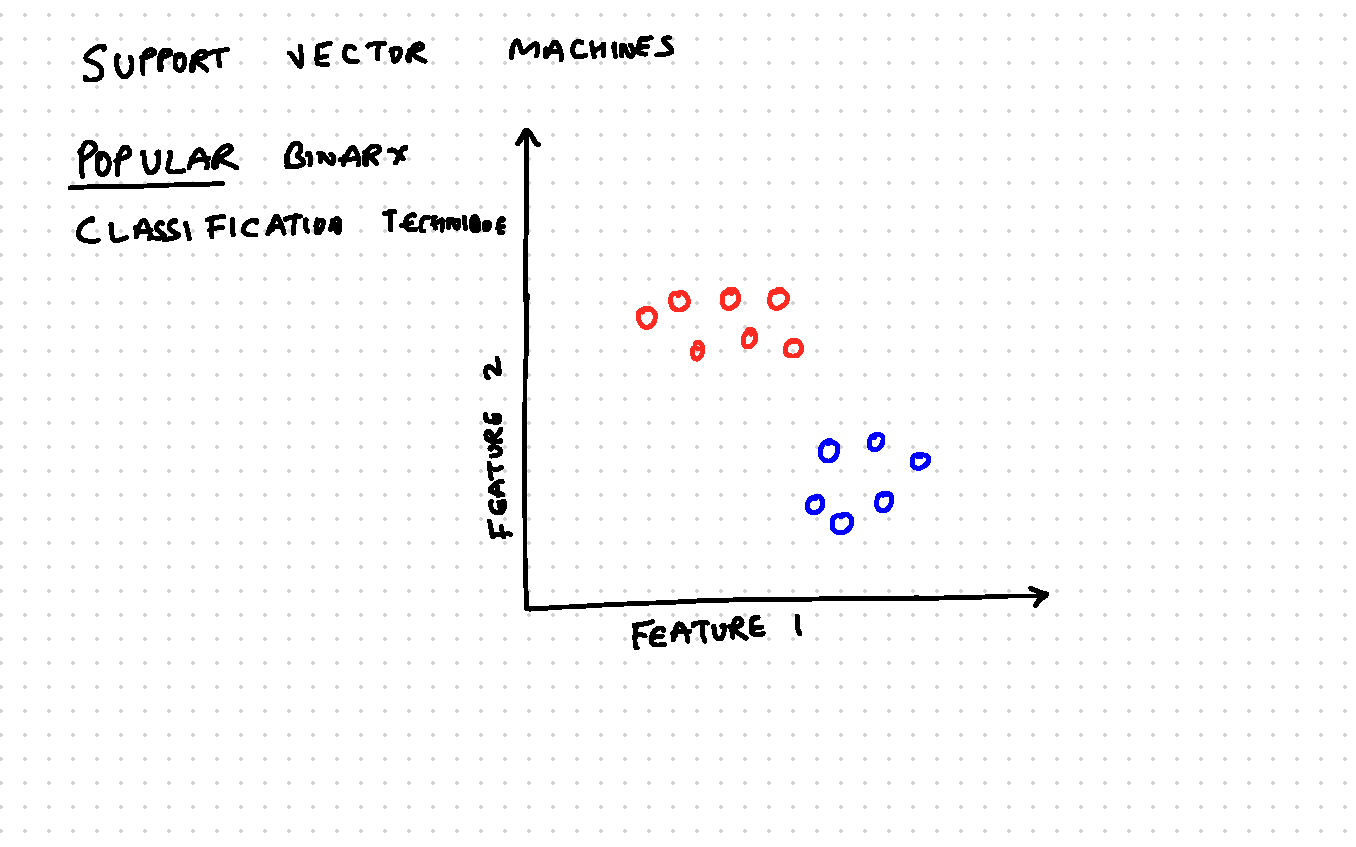
\includepdf[page=62]{Svm-notes.pdf}
}

	\begin{frame}{Loss Function for Sum (Hinge Loss)}
		Loss function is $\sum_{i=1}^{N}\max\big[0, 1 - y_{i}(\bar{w}\bar{x}_{i} + b)\big]$ \\
		\begin{itemize}[<+->]
			\item Case I 
			\hspace{0.5cm} $y_{i}(\bar{w}\bar{x}_{i} + b) = 1$ \\
			
			Lies on Margin: $Loss_{i}$ = 0 \\
		
			\item Case II \\
			\hspace{0.5cm} $y_{i}(\bar{w}\bar{x}_{i} + b) > 1$ \\
			$Loss_{i} = 0$ \\ 
			
			\item 	Case III \\
			\hspace{0.5cm} $y_{i}(\bar{w}\bar{x}_{i} + b) < 1$ \\
			$Loss_{i} \neq 0$
		\end{itemize}
		
		
	
	\end{frame}
	\begin{frame}{Hinge Loss Continued}
		Q) Is hinge loss convex and differentiable? \\
		\hspace{0.5cm}Convex: $\checkmark$ \\
		\hspace{0.5cm}Differentiable: X\\
		\hspace{0.5cm}Subgradient: $\checkmark$
	\end{frame}
	\begin{frame}{SVM Loss is Convex}
		
		Hinge Loss $\sum(\max[0, (1-y_{i}(\bar{w}x_{i}+b))]$ is convex \\
		\vspace{1cm}
		Penalty $\frac{1}{2}\lvert\lvert\bar{w}\rvert\rvert^{2}$ is convex \\
		\vspace{1cm}
		$\therefore$ SVM loss is convex
	\end{frame}
	
\end{document}